\documentclass{article}

\usepackage[utf8]{inputenc}
\usepackage{amsmath}
\usepackage{amssymb}
\usepackage{anysize}
\usepackage{color}
\usepackage{xcolor}
\usepackage{graphicx}
\usepackage{float}
\usepackage{subfigure}

\usepackage{listings}
\lstset{
	language=Matlab,                	% choose the language of the code
	keywords={break,case,catch,continue,else,elseif,end,for,function,
      global,if,otherwise,persistent,return,switch,try,while},
      keywordstyle=\color{blue},
      commentstyle=\color{red},
	basicstyle=\footnotesize,       % the size of the fonts that are used for the code
	numbers= left,                 	% where to put the line-numbers
	numberstyle=\footnotesize,      % the size of the fonts that are used for the line-numbers
	stepnumber=1,                   % the step between two line-numbers. If it is 1 each line will be numbered
	numbersep=5pt,                  % how far the line-numbers are from the code
	backgroundcolor=\color{white},  % choose the background color. You must add \usepackage{color}
	showspaces=false,               % show spaces adding particular underscores
	showstringspaces=false,         % underline spaces within strings
	showtabs=false,                 % show tabs within strings adding particular underscores
	frame=single,           		% adds a frame around the code
	tabsize=2,          			% sets default tabsize to 2 spaces
	captionpos=t,          			% sets the caption-position to bottom (t=top, b=bottom)
	breaklines=true,        		% sets automatic line breaking
	breakatwhitespace=false,    	% sets if automatic breaks should only happen at whitespace
	escapeinside={\%*}{*),  % if you want to add a comment within your code
	flexiblecolumns=true}         
}




\usepackage{caption}
\DeclareCaptionFont{white}{\color{white}}
\DeclareCaptionFormat{listing}{\colorbox{gray}{\parbox[c]{\textwidth}{#1#2#3}}}
\captionsetup[lstlisting]{format=listing,labelfont=white,textfont=white}

\setlength\parindent{0pt}
\setlength{\parskip}{10pt}

\marginsize{3cm}{2cm}{2cm}{2cm}

\title{Advanced Image Analysis\\
		Wavelet Homework}
\author{Emre Ozan Alkan\\
		\{emreozanalkan@gmail.com\}\\
		MSCV-5}
\date{\today}

\begin{document}
\maketitle

\section{Introduction}

In this homework, we investigated the wavelet transform and its applications in image denoising. We developed two functions. They are; j-level wavelet transform of an NxN image and inverse j-level wavelet transform of and NxN array of wavelet coefficients.

\section{Implementation}

In the implementation part, I created two matlab functions and a matlab script for test. Functions are: 'jLevelWaveletTransform' and 'inverseJLevelWaveletTransform', and script called 'RUNME'. 

\subsection{Wavelet Transform}

We developed a function to calculate wavelet coefficients. It takes 3 input arguments: an input image, the number of levels J, and low pass filter. It outputs an array of NxN wavelet coefficients. 

\begin{lstlisting}[label=waveletTransform, caption=jLevelWaveletTransform.m]	
function [ waveletCoefficients ] = jLevelWaveletTransform( image, J, lowPassFilter )
%JLEVELWAVELETTRANSFORM J-level wavelet transform
%   A Matlab function for computing the J-level wavelet transform of an NxN image (assume N is a power of 2).

if ~isempty(J) && J < 1
    error('J is not valid');
end

[row, col] = size(image);

if row ~= col
    error('Image should be NxN');
elseif mod(row, 2) || mod(col, 2)
    error('assume N is a power of 2');
end

% High Pass Filter
for ii = 1 : length(lowPassFilter)
    highPassFilter(ii) = lowPassFilter(ii) * power(-1, ii);
end

% Flip the high pass filter
highPassFilter = fliplr(highPassFilter);

% Initialization
waveletCoefficients = zeros(row, row);
temp = zeros(row, row);

for ii = 1 : row
    % Low Pass Filtering
    imageRowLowPass = pconv(lowPassFilter, image(ii, :));
    % Downsampling
    downSampledRowLow = imageRowLowPass(1 : 2 : length(imageRowLowPass));
    % High Pass Filtering
    imageRowHighPass = pconv(highPassFilter, image(ii, :));
    % Downsampling
    downSampleRowHigh = imageRowHighPass(1 : 2 : length(imageRowHighPass));
    % Storing rows for jth level
    temp(ii, :) = [downSampledRowLow, downSampleRowHigh];
end

for ii = 1 : col
    % Low Pass Filtering
    imageColLowPass = pconv(lowPassFilter, temp(:, ii)'); % temp used
    % Downsampling
    downSampledColLow = imageColLowPass(1 : 2 : length(imageColLowPass));
    % High Pass Filtering
    imageColHighPass = pconv(highPassFilter, temp(:, ii)'); % temp used
    % Downsampling
    downSampleColHigh = imageColHighPass(1 : 2 : length(imageColHighPass));
    % Output for jth level
    waveletCoefficients(:, ii) = [downSampledColLow, downSampleColHigh];
end

% Recursive Call for (j-1)th Level
if J > 1
    waveletCoefficients(1 : (row / 2), 1 : (col / 2)) = jLevelWaveletTransform(waveletCoefficients(1 : (row / 2), 1 : (col / 2)), J - 1, lowPassFilter);
end

end


\end{lstlisting}

\subsection{Inverse Wavelet Transform}

We also developed inverse wavelet transformation function that reconstructs images from wavelet coefficients. It takes 3 inputs: array of wavelet coefficients, the number of levels J and low pass filter. It outputs a reconstructed image.

\begin{lstlisting}[label=waveletTransform, caption=jLevelWaveletTransform.m]	
function [ reconstructedImage ] = inverseJLevelWaveletTransform( waveletCoefficients, J, lowPassFilter )
%INVERSEJLEVELWAVELETTRANSFORM Inverse J-level wavelet transform
%    Inverse J-level wavelet transform of an NxN array of wavelet coefficients.

if ~isempty(J) && J < 1
    error('J is not valid');
end

[row, col] = size(waveletCoefficients);

if row ~= col
    error('Image should be NxN');
elseif mod(row, 2) || mod(col, 2)
    error('assume N is a power of 2');
end

% High Pass Filter
for ii = 1 : length(lowPassFilter)
    highPassFilter(ii) = lowPassFilter(ii) * power(-1, ii);
end

% Flip the high pass filter
highPassFilter = fliplr(highPassFilter);

% Recursive Call for (j-1)th Level
if J > 1
    waveletCoefficients(1 : (row / 2), 1 : (col /2)) = inverseJLevelWaveletTransform(waveletCoefficients(1 : (row / 2), 1 : (col /2)), J - 1, lowPassFilter);
end

% Initialization
reconstructedImage = zeros(row, col);
temp = zeros(row, col);

for ii = 1 : col
    % Upsampling for cols
    downSampledLow = waveletCoefficients(1 : (col / 2), ii);
    upSampledLow = zeros(1, 2 * length(downSampledLow));
    upSampledLow(1 : 2 : length(upSampledLow)) = downSampledLow;
    % Upsampling for cols
    downSampledHigh = waveletCoefficients((col / 2) + 1 : col, ii);
    upSampledHigh = zeros(1, 2 * length(downSampledHigh));
    upSampledHigh(1 : 2 : length(upSampledHigh)) = downSampledHigh;
    % Low pass filter
    upSampledLow = pconv(lowPassFilter, fliplr(upSampledLow));
    % High pass filter
    upSampledHigh = pconv(highPassFilter, fliplr(upSampledHigh));
    % Storing constructed cols for jth level
    temp(:, ii) = fliplr(upSampledLow + upSampledHigh);
end

for ii = 1 : row
    % Upsampling for rows
    downSampledLow = temp(ii, 1 : (row / 2));
    upSampledLow = zeros(1, 2 * length(downSampledLow));
    upSampledLow(1 : 2 : length(upSampledLow)) = downSampledLow;
    % Upsampling for rows
    downSampledHigh = temp(ii, (row / 2) + 1 : row);
    upSampledHigh = zeros(1, 2 * length(downSampledHigh));
    upSampledHigh(1 : 2 : length(upSampledHigh)) = downSampledHigh;
    % Low pass filter
    upSampledLow = pconv(lowPassFilter, fliplr(upSampledLow));
    % High pass filter
    upSampledHigh = pconv(highPassFilter, fliplr(upSampledHigh));
    % Stroing reconstructed rows for jth level
    reconstructedImage(ii, :) = fliplr(upSampledLow + upSampledHigh);
end

end

\end{lstlisting}

\section{Results}

We used famous Lena image for tests. Forward and inverse wavelet transform applied on Lena with Daubechies D4 filter. Also we tested adding noise and using hard and soft thresholds. Results were reasonable for reconstruction. Here you see the results on the figures. 

\begin{figure}[h!]
	\centering
    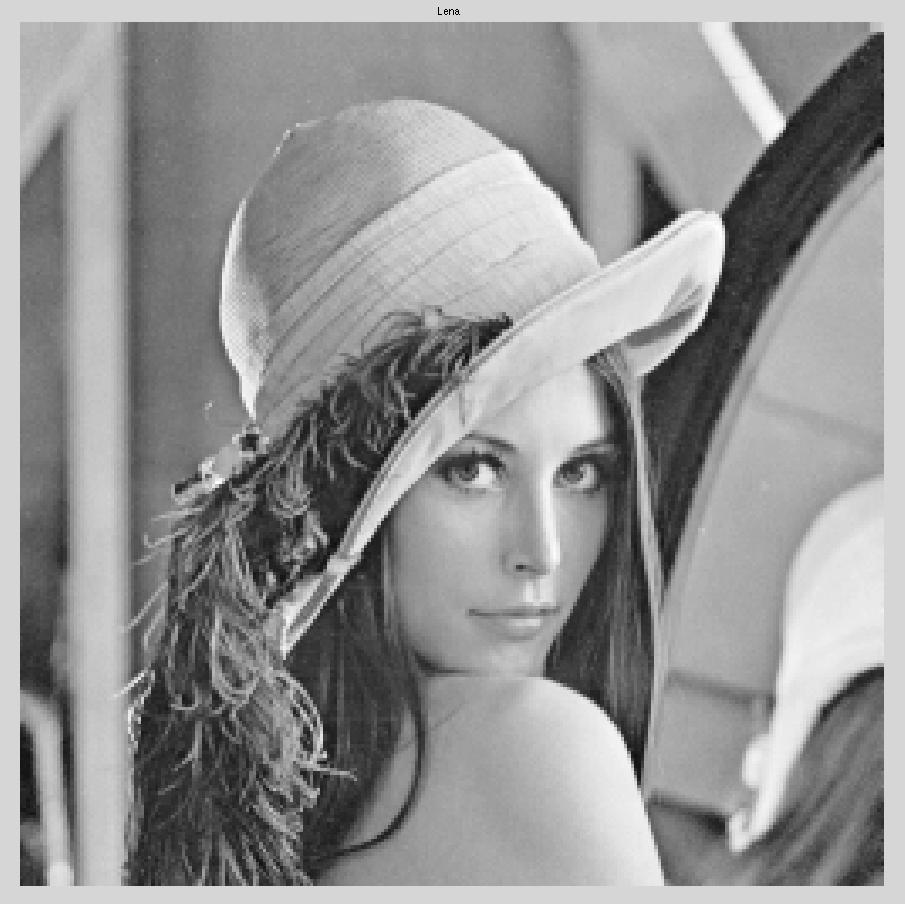
\includegraphics[width=0.5\textwidth]{../wavelet1}
    \caption{Lena Image}
\end{figure}

\begin{figure}[h!]
	\centering
    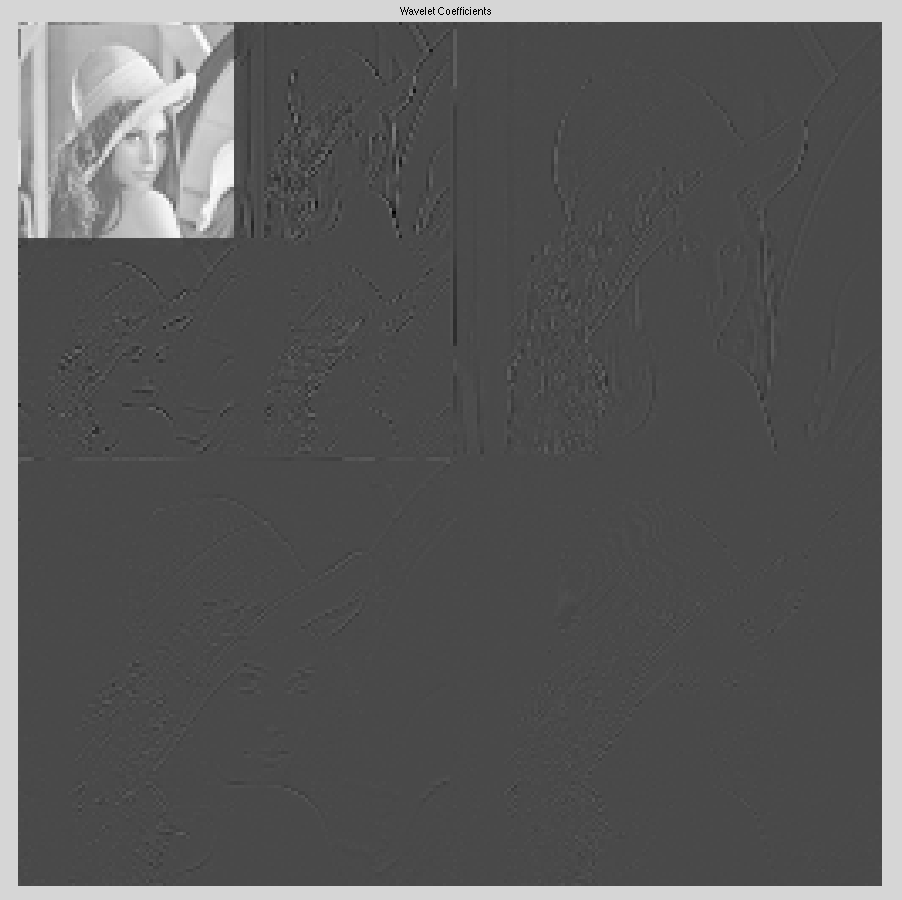
\includegraphics[width=0.5\textwidth]{../wavelet2}
    \caption{Lena Wavelet Coefficients}
\end{figure}

\begin{figure}[h!]
	\centering
    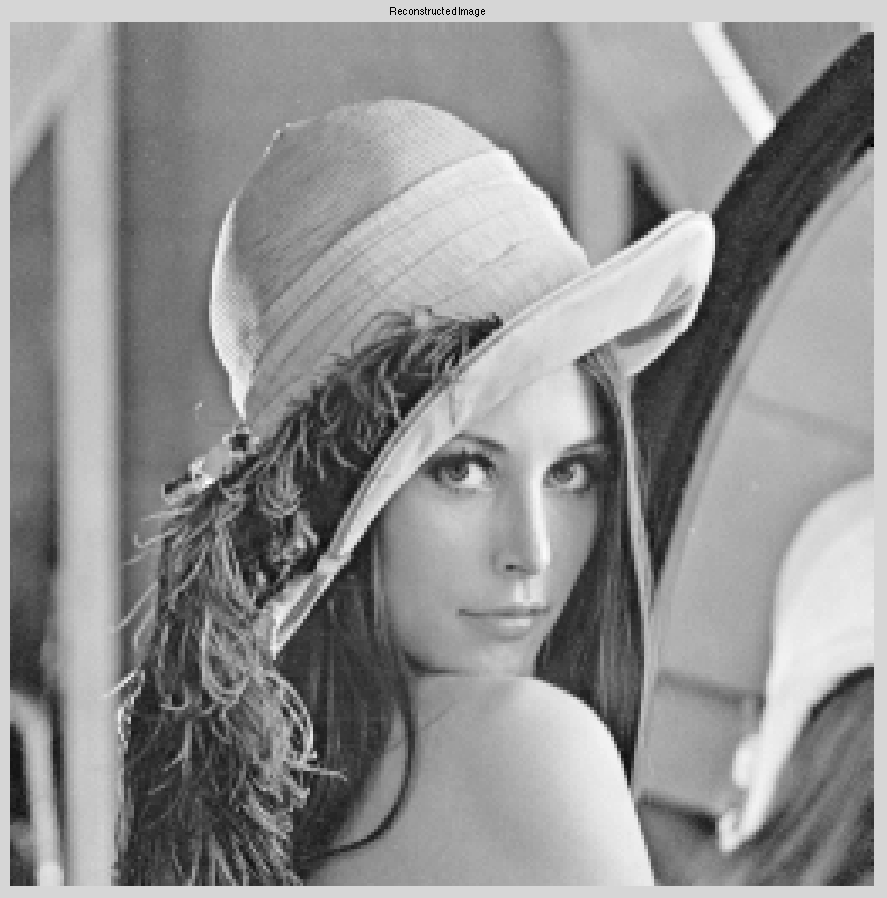
\includegraphics[width=0.5\textwidth]{../wavelet3}
    \caption{Lena Reconstructed from Wavelet Coefficients}
\end{figure}

\begin{figure}[h!]
	\centering
    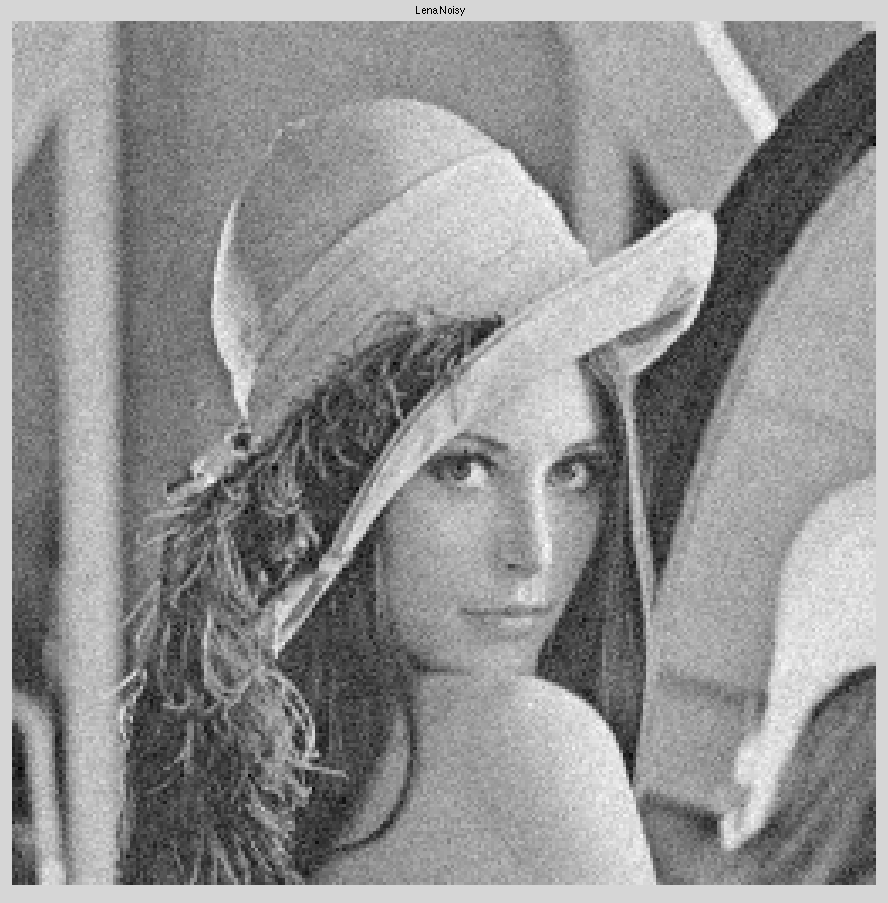
\includegraphics[width=0.5\textwidth]{../wavelet4}
    \caption{Lena Noise Added}
\end{figure}

\begin{figure}[h!]
	\centering
    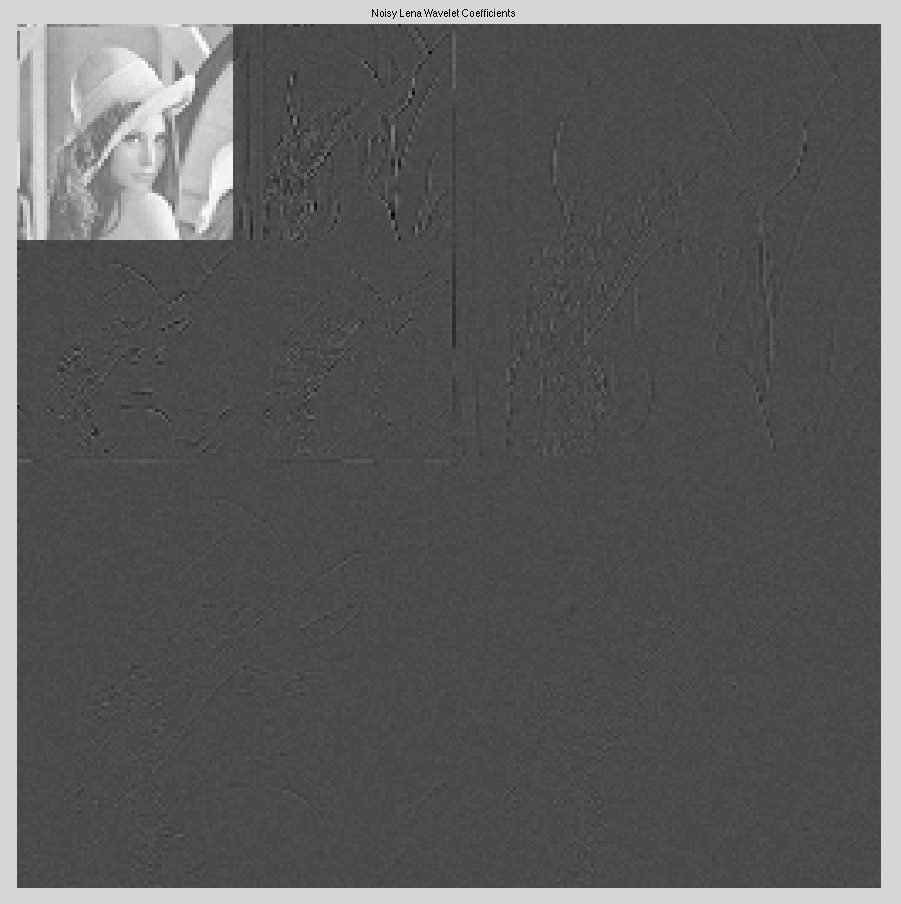
\includegraphics[width=0.5\textwidth]{../wavelet5}
    \caption{Noisy Lena Wavelet Coefficients}
\end{figure}

\begin{figure}[h!]
\centering
\subfigure[Soft Threshold]{
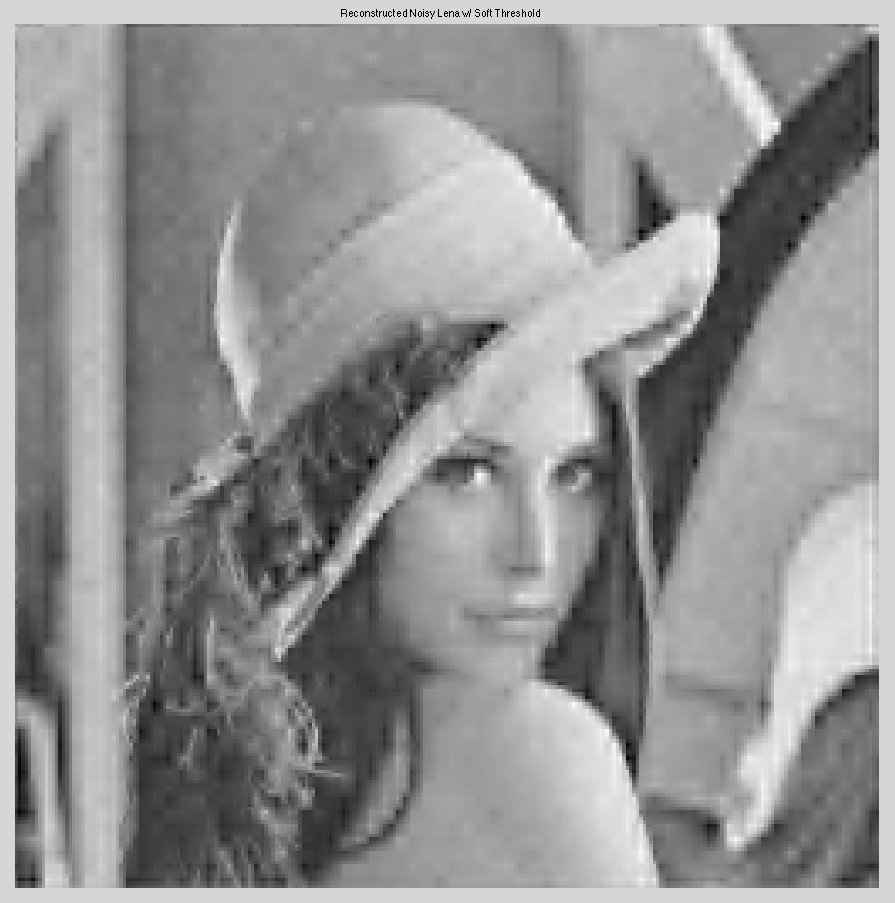
\includegraphics[width=.480\textwidth]{../wavelet6}
}
\subfigure[Hard Threshold]{
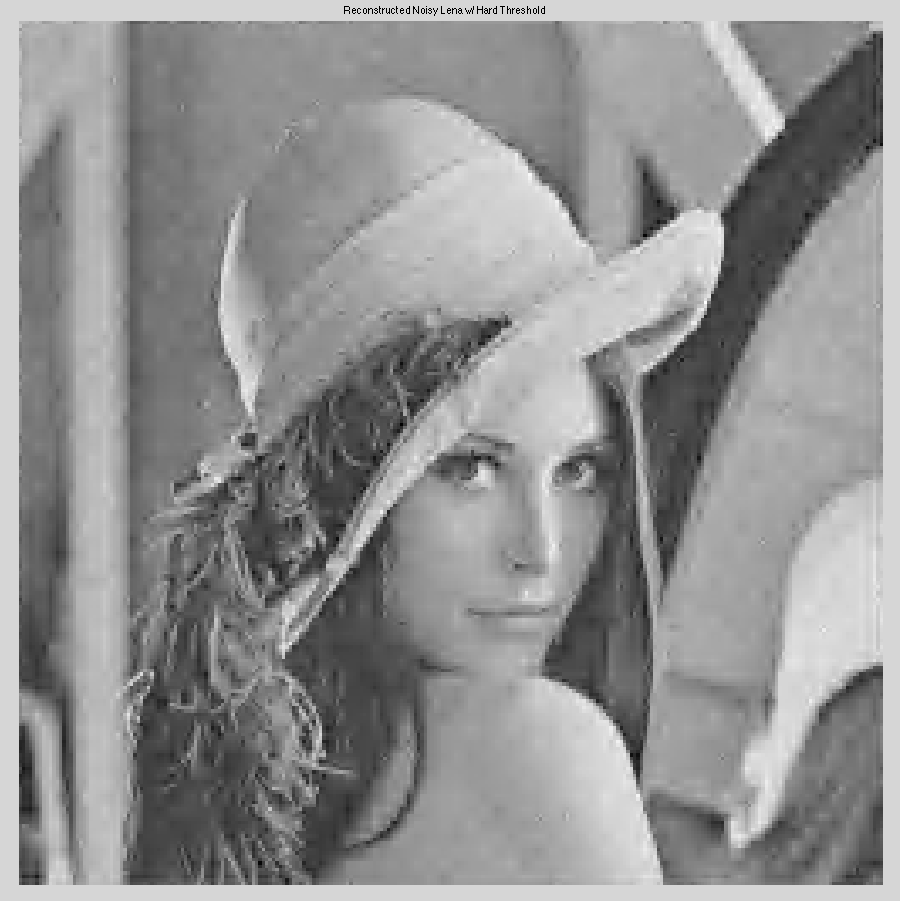
\includegraphics[width=.480\textwidth]{../wavelet7}
}
\caption{Noisy Lena Image Reconstructed with Threshold}
%\label{fig:whatever}
\end{figure}

%\begin{figure}[h!]
%	\centering
%    \includegraphics[width=0.5\textwidth]{../wavelet67}
%    \caption{Noisy Lena Wavelet Coefficients}
%\end{figure}

%\begin{figure}[H]
%\centering
%\subfigure[Control Law]{
%\includegraphics[width=.480\textwidth]{Control1}
%}
%\subfigure[Error]{
%\includegraphics[width=.480\textwidth]{Error1}
%}
%\caption{Control Law and Error Graph}
%%\label{fig:whatever}
%\end{figure}


%\begin{figure}[H]
%
%  \centering
%    \includegraphics[width=0.7\textwidth]{CameraPose21.png}    
%    
%     \caption{Loosing Feature: Camera Pose One Feature Lost}
%\end{figure}















\end{document}